In the above, we assumed that the parameters governing our model, $\vth=\{\alpha, \beta, \sig, \tau, \lam\}$, were known. In general, however, these parameters must be estimated from the data. Therefore, we take an approximate expectation-maximization approach for computing $\hbn$: (i) initialize some estimate of the parameters, $\hbth$, then (ii) recursively compute $\hbn$ using those parameters and update $\hbth$ given $\hbn$, and (iii) stop recursing when some convergence criteria is met.  Below, we provide details for each of the above steps.

\paragraph{Initializing the parameters}

We initialize our estimate $\balpha$ using Principal Component Analysis (PCA). More specifically, we perform PCA on $\bF$ (the whole movie), and let $\balpha$ be the PC with the highest eigenvalue.  If the movie is very long, we either only use part of it, or simply take the mean frame.  Then, we let $\beta=0$.  $\sig$ is estimated by finding a sequence of the time series lacking any obvious spikes, and computing the root mean square of that segment (i.e., $\hsig=\sqrt{\vF_{s:t}.^2}/(t-s)$).  We typically set $\gam$ and $\lam$ based on our previous experience with these cells.  For instance, $\gam \approx 0.95$ is often reasonable, and $\lam$ is somewhere between 1 and 10 Hz.  

\paragraph{Estimating the parameters given $\hbn$}

To find the maximum likelihood estimator for the parameters, $\hvth$, we must integrate over all possible spike trains. Unfortunately, it is not currently known how to perform this integral exactly, and approximating this integral using Monte Carlo methods is relatively time consuming (see \cite{VogelsteinPaninski09} for details).  Thus, we resort to a more drastic approximation, commonly used in state-space models.  For specifically, instead of integrating over all possibly spike trains, we only consider the most likely sequence (often referred to as the Viterbi path \cite{Rabiner89}): 

%\begin{subequations} \label{eq:par}
\begin{align} \label{eq:par1}
\widehat{\bth} &= \argmax_{\bth \in \ve{\Theta}} \int P[\bF|\bC, \bth] P[\bC | \bth]  d\bC  \approx \argmax_{\bth \in \ve{\Theta}}P[\bF| \hbC, \bth] P[\hbC, | \bth]
\end{align}

\noindent where $\hbC$ is determined using the above described inference algorithm. The approximation in \eqref{eq:par1} is good whenever the likelihood is very peaky, meaning that most of the mass is around the MAP sequence.\footnote{The approximation in \eqref{eq:par1} may be considered a first-order Laplace approximation}  

Due to the state space nature of the above model (Eqs \eqref{eq:bF} and \eqref{eq:C}), the optimization in Eq \eqref{eq:par1} simplifies significantly.  More specifically, we can write the argument from the right-hand-side of Eq \eqref{eq:par1} as a product of terms that we have defined in our model:

 \begin{align} \label{eq:par2}
P[\bF| \hbC, \bth] P[\hbC | \bth] &= \prod_{t=1}^T P[F_t | \hC_t; \balpha, \beta,\sig] P[\hC_t | \hC_{t-1}, \hn_t; \gamma] P[\hn_t | \lam].
\end{align}

\noindent This optimization simplifies into several separable problems.  %: (1) $\{\balpha, \beta\}$, (2) $\sig$, (3) $\gam$, and (4) $\lam$.  
First, we solve for $\balpha$ and $\beta$.  Because solving for them jointly is non-concave, we solve for each separately.  Consider $\balpha$ only:

\begin{subequations}
\begin{align}
\hbalpha 
&= \argmax_{\balpha} \prod_{t,x=1}^{T,N_p}  \p[F_{t,x} | C_t] 
=  \argmax_{\balpha} \prod_{t,x=1}^{T,N_p} \mN(F_{x,t}; \alpha_x ( C_t + \beta), \sig^2) \\
&= \argmax_{\balpha} \sum_{t,x=1}^{T,N_p} \log \mN (F_{x,t}; \alpha_x ( C_t + \beta), \sig^2)  \\
&= \argmax_{\balpha}  -\frac{N_p T}{2}\log(2\pi \sig^2) -\frac{1}{2\sig^2}\sum_{t,x=1}^{T,N} (F_{t,x} - \alpha_x(C_t + b))^2 \\
&= \argmin_{\balpha} \sum_{t,x=1}^{T,N_p} (F_{t,x} - \alpha_x(C_t + \beta))^2.
\end{align}
\end{subequations}

Therefore, we can solve for each of the $\halpha_x$'s separately and efficiently using Matlab's  \texttt{mldivide}: 
%
%\begin{align}
	$\halpha_x = (\bC + \beta\ve{1})\backslash \bF_x$, 
%\end{align}
%
where $\bF_x=[F_{1,x}, \ldots, F_{T,x}]\T$. Given $\hbalpha$, we can estimate $\beta$:

\begin{align}
\hbeta 
= \argmax_{\beta>0} \sum_{t,x=1}^{T,N} (F_{t,x} - \halpha_x(C_t + \beta))^2 
= \argmax_{\beta>0} \sum_{t,x=1}^{T,N} (F_{t,x} - \halpha_x C_t + \beta \halpha_x)^2 
\end{align}

\noindent which can again be solved efficiently again using Matlab's \texttt{mldivide}: $\widetilde{\beta}= \halpha_x \backslash \left(\sum_{t=1}^T F_{t,x} - \halpha_x C_t\right)$.  If $\widetilde{\beta}<0$, we simply let $\hbeta=0$, else, $\hbeta=\widetilde{\beta}$.

Given $\hbalpha$ and $\hbeta$, we can now estimate $\sig$ using the residuals, i.e.,

\begin{align}
	\hsig^2 = \frac{1}{T N_p}\norm{\vec{\bF} - \hbalpha(\bC\T + \beta \ve{1})}^2
\end{align}

Estimating $\lam$ is also totally straightforward: $\widehat{\lam} = \hbn' \ve{1}/ (T \Del)$. 
% 
% \begin{align} 
% \widehat{\lam} &=  \frac{1}{T \Del} \hbn' \ve{1} \label{eq:lam}
% \end{align}

We don't update $\gam$ as we have found that it does not improve inference quality (not shown), in agreement with previous work \cite{YaksiFriedrich07}.

%\paragraph{Convergence criteria}

We stop iterating the parameter update whenever (i) iteration number exceeds some upper bound, or (ii) relative change in likelihood does not exceed some lower bound.  In practice, we find that parameters tend to converge after several iterations, given our initialization.  Figure \ref{fig:spatial_EM} shows a simulation demonstrating the efficacy of this procedure.  The left panel shows the true spatial filter (top), the 1-dimensional fluorescence projection using the true spatial filter, $\bF^{opt}$ (middle), and the inferred spike train using the true parameters (bottom).  The right panel shows the estimated spatial filter, the 1-dimensional fluorescence projection using the estimated filter, $\bF^{est}$, and the inferred spike train using the estimated filter.  Note that we seeded the algorithm with the movie, and parameter estimates that were at least a factor of 2 from the true values.

\begin{figure}[h!]
\centering 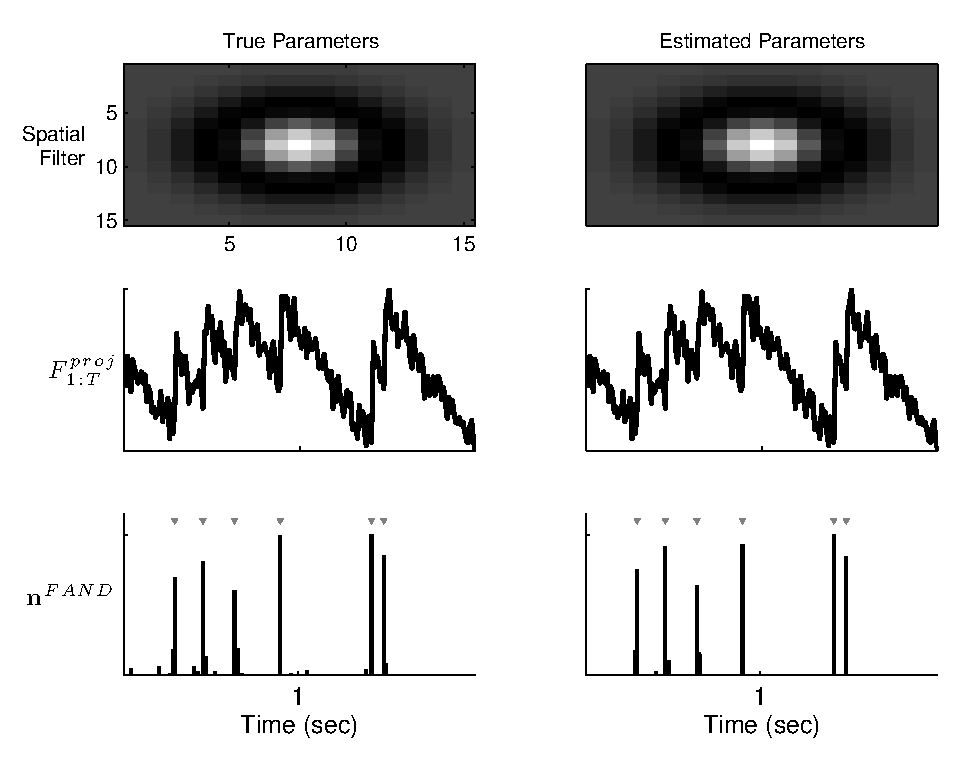
\includegraphics[width=.9\linewidth]{../figs/spatial_EM}
\caption{A simulation demonstrating that given only the fluorescence movie, the parameters may be estimated, and the spike train inferred (c.f. Supplementary Movie 2). Top left panel: true spatial filter.  Middle left panel: projection of movie onto true spatial filter. Bottom left panel: inferred spike train using true parameters. Right panels: same as left except estimating parameters.  All parameters estimated other than $\gam$, which was assumed known.  Parameters converged within 7 iterations.  Simulation details: $T=1000$, $\Del=5$ msec, $\balpha$ is the same as in Figure \ref{fig:spatial}, $\beta=0$, $\tau=500$ msec, $\lam=10$ Hz.} \label{fig:spatial_EM}
\end{figure}

%we solve:
%
%\begin{align} 
%\{\halpha, \hbeta, \hsig\} &= \argmax_{\balpha, \beta, \sig > 0} \sum_{t=1}^T \log P[F_t | \hC_t, \balpha, \beta, \sig] \nonumber \\
%&=  \argmax_{\balpha, \beta, \sig > 0} -\frac{T}{2} \log (2 \pi \sig^2)  - \frac{1}{2\sig^2} \sum_{t=1}^T (F_t - \balpha \hC_{t} - \beta )^2 \nonumber \\
%&=   \argmax_{\balpha, \beta, \sig > 0} -\frac{T}{2} \log (2 \pi \sig^2)  - \frac{1}{2\sig^2} \norm{\bF- \hbX \ve{\eta}}^2 \label{eq:lik2}
%%P[\bF | \hbC, \balpha, \beta, \sig) &= \prod_{t=1}^T P[F_t | \hC_t, \balpha, \beta, \sig) = \prod_{t=1}^T \frac{1}{\sqrt{2 \pi \sig^2}} \exp \left\{-\frac{1}{2\sig^2} (F_t - \balpha \hC_t - \beta )^2\right\}, \label{eq:lik}% \nonumber \\
%%&= \prod_{t=1}^T \frac{1}{\sqrt{2 \pi \sig^2}} \exp \left\{-\frac{1}{2\sig^2} \big[F_t - \balpha (\gamma \hC_{t-1} + n_t) - \beta \big]^2\right\} \label{eq:lik}
%\end{align}
%
%%\noindent which follows from Eq \eqref{eq:trans}. Taking the log of both sides yields:
%%
%% because $\hC_t$ is deterministic given $\hn_t$. Considering for a moment, only the quadratic term in Eq \eqref{eq:lik}, the terms can be reorganized:
%%
%%\begin{align}
%%F_t - \balpha (\gamma \hC_{t-1} + \nu + \rho \hn_t) - \beta &= F_t - (\balpha \gamma) \hC_{t-1} - (\balpha \nu + \beta) - (\balpha \rho) \hn_t 
%%\end{align}
%%
%%\noindent which emphasizes the over-parameterization in our model.  Thus, without loss of generality, we can assume that $\balpha=1$ and $\beta=0$. Taking logs in Eq \eqref{eq:lik} then yields:
%%
%%\begin{align} 
%%\log P[\bF | \hbn, \bth) &=  -\frac{T}{2} \log (2 \pi \sig^2)  - \frac{1}{2\sig^2} \sum_{t=1}^T (F_t - \balpha \hC_{t} - \beta )^2 \nonumber \\
%%&=  -\frac{T}{2} \log (2 \pi \sig^2)  - \frac{1}{2\sig^2} \norm{\bF- \hbX \ve{\eta}}^2
%% \label{eq:lik2}
%%\end{align}
%
%\noindent where  $\ve{\eta}=[\balpha, \, \beta]$  and $\hbX_t=[\hC_{t}, \, 1]$.  Thus, solving for $\{\halpha,\hbeta\}$, is a constrained quadratic optimization problem, which can be solved efficiently using standard tools, such as Matlab's \texttt{quadprog}.  The variance may then be solved for analytically:
%
%\begin{align} 
%\widehat{\sig}^2 &= \frac{1}{T} \norm{\bF - \hbX \widehat{\ve{\eta}}}_2^2 \label{eq:sig}
%\end{align}
%
%\noindent Similarly, taking the log of the prior term, $P[\hbn | \bth )$ yields:
%
%\begin{align} \label{eq:prior}
%\log P[\hbn | \bth] =  \sum _{t=1}^T \log(\lam \Del)  -\lam \Del \hn_t =T (\lam \Del) - \lam \Del \hbn' \ve{1} 
%\end{align}
%
%\noindent Plugging Eqs \eqref{eq:lik2} and \eqref{eq:prior} back into Eq \eqref{eq:par1}, and noting that log is a monotonic function, we have:
%
%
%%Given Eqs. \eqref{eq:obs} and \eqref{eq:trans}, we can write the above likelihood function as:
%
%\begin{align} 
%%\hvth &=\argmax_{\vth \in \ve{\Theta}}  \sum_{t=1}^T \left(- \frac{1}{2} \log (2\pi\sig^2)-\frac{1}{2\sig^2} (F_t - \gamma \hC_{t-1} -\nu  - \rho \hn_t)^2 \right) + \sum_{t=1}^T \big(\log (\lam \Del) -  \lam \Del n_t\big) \nonumber \\
%\hvth &=\argmax_{\vth \in \ve{\Theta}} - \frac{T}{2} \log (2\pi\sig^2) - \frac{1}{2\sig^2} \norm{\bF - \hbX \ve{\eta}}_2^2 + T \log (\lam \Del) - \lam \Del \hbn' \ve{1} \label{eq:par} 
%%&=\argmin_{\vth}  \frac{T}{2} \log (2\pi\sig^2)  +  \frac{1}{2\sig^2} \norm{\bY + \ve{\eta} \bX}_2^2 + T \log (\lam \Del) - \lam \Del \bn' \ve{1} \label{eq:par} 
%\end{align}
%%\end{subequations}
%
%\noindent %where %$\bY=\bF- \hbn$, 
%%$\bX=[\hbC, \,  \ve{1},\,  \hbn]'$, $\ve{\eta}=[\gamma, \nu, \rho]'$, and $\hbC=[\hC_1, \hC_2, \ldots, \hC_{T-1}]'$ is the inferred calcium concentration using the algorithm described in Section \ref{sec:inf} (and $\hbn$ is defined in a similar fashion). Note that had we not fixed $\balpha=1$ and $\beta=0$, then we would have had $\ve{\eta}=[\balpha \gamma, \balpha \nu + \beta, \balpha \nu]$, and then these parameters would not have been identifiable.  
%Estimating the parameters then separates into three log-concave problems.  In particular, solving for $\widehat{\ve{\eta}}$ is simply:
%
%\begin{align} 
%\widehat{\ve{\eta}} &= \argmin_{\ve{\eta},\: 0< \eta_1<1} \frac{1}{2} \norm{\bF - \hbX \ve{\eta}}_2^2 
%=  \argmin_{\ve{\eta},\: 0< \eta_1<1} \frac{1}{2} \ve{\eta}' \bQ  \ve{\eta} - \bL'  \ve{\eta} \label{eq:m} 
%\end{align}
%
%\noindent where $\bQ=\hbX' \hbX$, and $\bL=\hbX' \bF$, and the constraint, $0<\eta_1<1$, ensures that the time constant is both non-negative and finite.  Eq \eqref{eq:m} may be solved using standard quadratic optimization tools, such as Matlab's \texttt{quadprog}.  
%
%Unfortunately, the recursive nature of our algorithm makes solving for $\hbeeta$ in this manner unidentifiable. In particular, because both $\hbX$ and $\beeta$ can scale and shift $\bC$, alternating between inferring $\hbX$ and $\hbeeta$ does not converge (data not shown). However, this is not particularly problematic, because the fluorescence measurements are in arbitrary units. This unit arbitrariness suggests that $\bF$ may be scaled and shift without loss of generality. The prior term and non-negativity constraint on $\bn$, however, imposes small costs associated with scaling and shifting $\bn$ and $\bC$.  We therefore estimate $\beeta$ from the raw fluorescence trace.  More specifically, to estimate $\gamma$, we manually find a fluorescence sequence that seem to be decaying, estimate the time constant $\tau$, and let $\gamma=1-\Del/\tau$.  For $\nu$, we manually find a fluorescence sequence that seems to be near baseline, label it $[F_s,\ldots, F_t]$, and let $\nu=\frac{1}{t-s}\sum_{u=s}^t F_u$.  Finally, we estimate $\rho$ by letting it be equal to what we manually determine it be, by eye.  In practice, we have found that by first scaling and shifting $\bF$ to be between $0$ and $1$, subsequent traces from the same or different cells have very similar values for $\beeta$, and therefore, these parameters need not be tweaked much.  Furthermore, the effective signal-to-noise ratio (SNR) of the inferred spike train does not depend strongly on these parameters, in agreement with previous results \cite{YaksiFriedrich06}.  The other parameters, $\sig$ and $\lam$, can be solved for analytically:
%
%\begin{align} 
%\widehat{\sig}^2 &= \frac{1}{T} \norm{\bF - \hbX \widehat{\ve{\eta}}}_2^2 \label{eq:sig2}\\
%\widehat{\lam} &=  \frac{1}{T \Del} \hbn' \ve{1} \label{eq:lam}
%\end{align}
%
%
%initialize: use approximate pca algorithm
%
%recursion: solve for $\balpha$ first, then $\beta$
%
%stopping criteria: likelihood stops improving significantly
%
%Note that we can expand
%\begin{align}
%\p[\bF | \bC] 
%= \prod_{t=1}^T \p[\bF_t | C_t] 
%= \prod_{t=1}^T \prod_{x=1}^N \p[F_{t,x} | C_t] 
%\end{align}
%
%
%
%%In the above, we assumed a one-dimensional (1-D) observation, $\bF$.  The raw data, however, is actually a series of multidimensional images. To get the 1-D time-series, two pre-processing steps are required.  First, for each neuron, one must define a region-of-interest (ROI), essentially assigning sets of pixels to neurons. This yields a vector time-series for each neuron, $\vbF_t \in \Real^m$.   Second, one must project the $m-$D observations into a 1-D time-series.  Typically, this step is performed by averaging all the pixels within the ROI.  In theory, one can improve on this uniform averaging by estimating the optimal spatial filter. Here, we provide details on how to incorporate this second step (projecting the $m-$D observations into 1-D) into our \foopsi filter. First, we replace Eq \eqref{eq:obj} with:
%%
%%\begin{align}
%%\vbF_t &= \ve{\balpha} C_t + \ve{\beta} +  \ve{\Sig} \ve{\varepsilon}_t, \qquad \varepsilon_t \sim \mathcal{N}(\ve{0},\bI) \label{eq:Obs} 
%%\end{align}
%%
%%\noindent where $\vbF_t$, $\ve{\balpha}$, and $\beta$ are all $m$ dimensional column vectors, $\ve{\Sig}$ is the covariance matrix, and $\ve{\varepsilon}_t$ is an $m-$dimensional standard normal random vector. $\Alpha$ now represents the optimal spatial filter, and $\Beta$ represents the baseline for each pixel.  Our goal then is to estimate $\Alpha$ and $\Beta$, to provide maximal information about the underlying spike train.  We would expect this optimal spatial filtering improve the effective SNR after filtering in many situations.  For example, if certain pixels are anti-correlated with others, a uniform spatial filter would average out those differences, whereas the optimal filter would take advantage of that information.    
%%
%%To estimate $\Alpha$ and $\Beta$, we first plug 
%%Then, plugging %To estimate the optimal spatial filter, first we assume that both $\bn$ and $\bC$ are known.  Then, letting $\ve{\eta}_v=[\gam \ve{\Alpha}, \nu \Alpha + \Beta, \rho \Alpha]'$, we see that the parameters are again unidentifiable.  This time, we let $\nu=0$ and $\rho=1$, yielding $\ve{\eta}_v=[\gam \ve{\Alpha}, \Beta,\Alpha]'$.  Then, plugging 
%%Eqs \eqref{eq:Obs} and \eqref{eq:trans} into \eqref{eq:par1}, to obtain:
%%
%%\begin{align} 
%%\vec{\bth} &=\argmax_{\vec{\bth} \in \vec{\bTh}} - \frac{T}{2} \log (2\pi|\ve{\Sig}|) + T\log (\lam \Del) -  \lam \Del \bn' \ve{1} \nonumber\\
%%&-\frac{1}{2} \sum_{t=1}^T (\vbF_t - \ve{\balpha} (\gamma \hC_{t-1} -\nu  - \rho \hn_t) - \ve{\beta})' \ve{\Sig}^{-1} (\vbF_t - \ve{\balpha} (\gamma \hC_{t-1} -\nu  - \rho \hn_t) - \ve{\beta}) %\nonumber \\
%%\end{align} 
%%
%%\noindent where $| \cdot |$ indicates the determinant. By pre-whitening the observation matrix, $\vbF=[\vbF_1, \vbF_2, \ldots, \vbF_T]$, we can estimate the covariance matrix by the identity, i.e., $\ve{\Sig}=\ve{I}$.   Without loss of generality, we may assume that $\nu=0$ and $\rho=1$, similar to our assumption of $\balpha=1$ and $\beta=0$ above. This leaves $\gamma$, $\Alpha$, and $\Beta$. Assuming that $\gamma$ is known (or estimated from the raw fluorescence signal, as we did above), we have: 
%%
%%\begin{align}
%%\widehat{\ve{\eta}}_v = \argmax_{\norm{\ve{\eta}_v} <1} \norm{\vbF - \ve{\eta}_v \bX_v}^2 \label{eq:Par}
%%\ve{\eta}_v &=\argmax_{\ve{\eta}_v, \, 0 < \gamma < 1} %- \frac{T}{2} \log (2\pi|\ve{\Sig}|) + T \log (\lam \Del) -\lam \Del \bn'\ve{1} 
%%-(\vbF -\ve{\eta}_v \bX_v) ' \ve{\Sig}^{-1}   (\vbF - \bX \bth_v) \label{eq:Par}
%%\end{align}
%%
%%\noindent where $\ve{\eta}_v=[\Alpha, \, \Beta]$, and $\bX_v=[\gamma \bC + \bn, \, \ve{1}]'$. Note that we have constrained the norm of $\ve{\eta}_v$, which is necessary because otherwise there is a free scale between $\bX_v$ and $\ve{\eta}_v$.  Problems of the form as in Eq \eqref{eq:Par} are known as ``trust region subproblems''.  Fortunately, many algorithms for solving such a problem are available \cite{Fortin00}. 
%
%
%
%%\noindent where Eq. \eqref{eq:m} may be solved using standard linearly constrained quadratic programming (the constraint ensures that the time constant is both non-negative and finite), and the other two may be solved analytically. Importantly, when $\bn$ is unknown, $\widehat{\ve{\eta}}$ is not identifiable, as $\bY$ and $\ve{\eta}$ can both modify the offset and scale of $\bn$. Thus, we estimate $\ve{\eta}$ \emph{before} doing the analysis, and then hold it fixed throughout.  
%
%%. Because the noise is Gaussian, $a$ and $\beta$ may be estimated using standard constrained quadratic programming:
%% 
%%\begin{subequations}
%%\begin{align} \label{eq:m}
%%\{\ha,\hbeta\}% &= \argmax_{a,\beta>0}\frac{1}{\sqrt{2 \pi} \sig} \exp \left\{ -\frac{1}{2} \left(\frac{F_t - a \widehat{C}_{t-1} - \widehat{n}_t - \beta}{\sig}\right)^2\right\} 
%%= \argmin_{a,\beta>0} \sum_{t=1}^T (F_t - a \widehat{C}_{t-1} - \widehat{n}_t -\beta )^2 \\
%%\widehat{\ve{\eta}} &= \argmin_{\bm>0} \norm{\bY + \bm \bX}_2^2. % = \argmin_{\bm>0}  \bm' \bX' \bX \bm  - 2 \bY' \bX \bm 
%%\end{align}
%%\end{subequations}
%%
%% Similarly, because $\varepsilon_t$ is Gaussian, we compute $\widehat{\sig}$ analytically using: 
%%
%%\begin{align}
%%\widehat{\sig}^2 = \frac{1}{T} \norm{\bY + \widehat{\ve{\eta}} \bX}_2^2.
%%\end{align}
%%
%%\noindent The parameter for the prior term is given by:
%%
%%\begin{align}
%%\widehat{\lam} = \argmax_{\lam} P[\widehat{\ve{n}} | \lam) =  \argmax_{\lam} \log P[\widehat{\ve{n}} | \lam) =  \frac{T}{ \Del \bn' \ve{1}}
%%\end{align}
%%
%%\noindent which follows from assuming that $p(\zT | \lT)$ is exponential in \eqref{eq:approx}.
%
%
